\chapter{Аналитическая часть}

В данном разделе проводится сравнительный анализ методов решения
поставленной задачи, делается обоснованный выбор метода.

\section{Постановка задачи}

В соответствии c заданием необходимо разработать программное обеспечение для удаленного подключения к терминалу: серверное и клиентское приложение. Сервер должен поддерживать связь с множеством клиентов одновременно, обрабатывая запросы от каждого и рассылая изменения всем остальным. По необходимости сервер должен запустить команду терминала, высылая результат всем подключенным клиентам. Для решения этой задачи необходимо изучить предметную область и проанализировать существующие решения.

\section{Анализ существующих решений}

\subsection{tty-share}

\texttt{tty-share} \cite{tty-share} - инструмент, используемый для совместного редактирования терминала. Сеансом можно поделиться как в локальной сети, так и в удаленной. При совместном использовании терминала через сеть Internet, tty-share подключается к прокси-серверу, который является посредником при обмене данными между участниками. Экземпляр этого сервера может быть размещен как на вашей машине, так и на \texttt{tty-share.com}. Сквозное шифрование при таком подключении отсутствует.

К достоинствам tty-share можно отнести:
\begin{itemize}
	\item возможность подключения к сессии из браузера;
	\item отсутствие зависимостей. tty-share представляет из себя статический кроссплатформенный двоичный файл, который не содержит зависимостей;
\end{itemize}

\subsection{tmate}

\texttt{tmate} \cite{tmate} -- ответвление терминального мультиплексора tmux \cite{tmux}, который обеспечивает безопасное, мгновенное и простое в использовании решение для совместного использования терминалов с помощью ssh-соединения \cite{ssh}. На рисунке \ref{fig:tmux} представлена схема архитектуры tmate с различными компонентами.

\begin{center}
	\begin{figure}[H]
		\begin{center}
			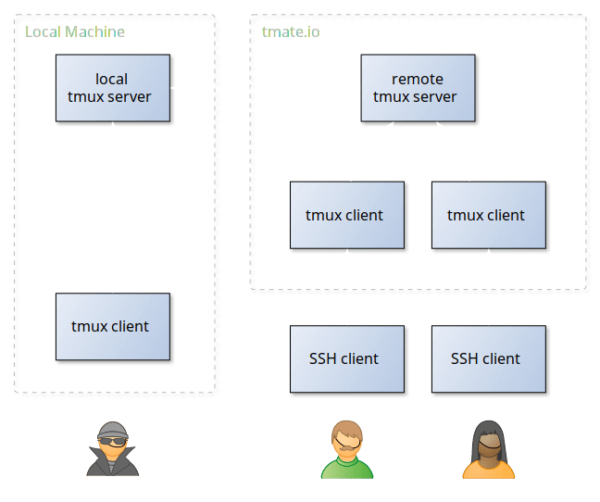
\includegraphics[scale=0.32]{img/tmate.png}
		\end{center}
		\caption{\label{fig:tmux} Схема архитектуры tmate. Слева представлена архитектура при запуске в локальной сети, справа -- в удаленной сети}
	\end{figure}
\end{center}

Локальный, как и удаленный сервер tmux взаимодействует с протоколом поверх стерилизатора данных msgpack \cite{msgpack}, который сжимается через ssh-соединение для повышения эффективности пропускной способности сети \cite{tmate}.

К достоинствам tmate можно отнести:
\begin{itemize}
	\item возможность подключения как в локальной сети, так и в удаленной;
	\item использование ssh-сессий;
	\item возможность разместить tmate-сервер как на своей машине, так и на серверах \texttt{tmate.io}.
\end{itemize}

\section{Модель клиент-сервер}

В модели клиент-сервер роли определены: сервер предоставляет ре­сурсы и службы одному или нескольким клиентам, которые обращаются к серверу за обслуживанием. В качестве примеров серверов можно привести веб­-серверы, почтовые серверы и файловые серверы . Каждый из этих серверов предоставляет ресурсы для клиентских устройств, таких как настольные ком­пьютеры, ноутбуки, планшеты и смартфоны . Большинство серверов могут устанавливать отношение <<один ко многим>> с клиентами, что означает, что один сервер может предоставлять ресурсы нескольким клиентам одновремен­но. Когда клиент запрашивает соединение с сервером, сервер может либо принять, либо отклонить это соединение. Если соединение принято, сервер устанавливает и поддерживает соединение с клиентом по определенному про­токолу. Например, почтовый клиент может запросить SMTP-соединение с почтовым сервером для отправки сообщения. Затем приложение SMTP на почтовом сервере запросит проверку подлинности у клиента, например адрес электронной почты и пароль. Если эти учетные данные совпадают с учетной записью на почтовом сервере, сервер отправит электронное письмо целевому получателю. Часто клиенты и серверы взаимодействуют через компьютерную сеть на разных аппаратных средствах, но и клиент и сервер могут находиться в одной и той же системе. Хост сервера запускает одну или несколько серверных программ, которые совместно используют свои ресурсы с клиентами. Клиент не предоставляет общий доступ ни к одному из своих ресурсов, но запраши­вает данные или службу у сервера. Поэтому клиенты инициируют сеансы связи с серверами, которые ожидают входящих запросов. Клиенту не знает о том, как работает сервер при выполнении запроса и доставке ответа. Клиент должен только понимать ответ, основанный на хорошо известном прикладном протоколе, т.е. содержание и форматирование данных для запрашиваемой службы. Клиенты и серверы обмениваются сообщениями в шаблоне обмена сообщениями запрос-ответ. Клиент отправляет запрос, а сервер возвращает ответ.

\section{Сокеты}

Сокет (англ. socket \cite{socket})— конечный пункт передачи данных, абстракция, обозначающая одно из окончаний сетевого соединения. Каждая из программ, устанавливаю­ щих соединение, должна иметь собственный сокет. Сокеты – это интерфейс прикладного программирования для сетевых приложений TCP/IP. Интерфейс сокетов был создан в восьмидесятых годах для операционной системы UNIX. Позднее интерфейс сокетов был перенесен в Microsoft Windows. Сокеты до сих пор используются в приложениях для сетей TCP/IP. Сетевые приложения используют сокеты, как виртуальные разъемы для обмена данными между собой. Сокеты бывают трех видов: клиентские, слушающие и серверные.

\subsection{Принципы сокетов}

Каждый процесс может создать слушающий сокет (серверный сокет) и привязать его к какому-нибудь порту операционной системы (в UNIX непри­вилегированные процессы не могут использовать порты меньше 1024). Слуша­ющий процесс обычно находится в цикле ожидания, то есть просыпается при появлении нового соединения. При этом сохраняется возможность проверить наличие соединений на данный момент, установить тайм-аут для операции и т.д.
Каждый сокет имеет свой адрес. ОС семейства UNIX могут поддержи­вать много типов адресов, но обязательными являются INET-адрес и UNIX­ адрес. Если привязать сокет к UNIX-адресу, то будет создан специальный файл (файл сокета) по заданному пути, через который смогут сообщаться любые локальные процессы путём чтения/записи из него. Сокеты типа INET доступны из сети и требуют выделения номера порта \cite{socket-nets-programming}.
Обычно клиент явно подсоединяется к слушателю, после чего любое чтение или запись через его файловый дескриптор будут передавать данные между ним и сервером.

\subsection{Основные функции сокетов}

В таблицах \ref{tab:socket_main} - \ref{tab:socket_client} представлены общие функции, функции сервера и клиента соотвественно.

\begin{table}[h]
	\begin{center}
		\begin{tabular}{ |c|c| }
			\hline 
			Функция & Описание \\  \hline
			\texttt{socket} & Создать новый сокет и вернуть файловый дескриптор \\ \hline
			\texttt{send} & Отправить данные по сети \\ \hline 
			\texttt{receive} & Получить данные по сети \\ \hline 
			\texttt{close} & Закрыть соединение \\ \hline
		\end{tabular}
		\caption{\label{tab:socket_main} Общие функции}
	\end{center}
\end{table}

\begin{table}[h]
	\begin{center}
		\begin{tabular}{ |c|c| }
			\hline 
			Функция & Описание \\  \hline
			\texttt{bind} &  Связать сокет с IP-адресом и портом \\ \hline
			\texttt{listen} & Слушает порт и ждет когда будет установлено соединение\\ \hline 
			\texttt{accept} & Принять запрос на установку соединения \\ \hline 
		\end{tabular}
		\caption{\label{tab:socket_server} Функции сервера}
	\end{center}
\end{table}

\begin{table}[h]
	\begin{center}
		\begin{tabular}{ |c|c| }
			\hline 
			Функция & Описание \\  \hline
			\texttt{connect} & Установить соединение \\ \hline
		\end{tabular}
		\caption{\label{tab:socket_client}Функции клиента}
	\end{center}
\end{table}

\subsection{Типы сокетов}

Различают два типа сокетов:

\begin{itemize}
	\item[---] сокеты с предварительным установлением соединения, когда до начала передачи данных устанавливаются адреса сокетов отправителя и получателя данных – такие сокеты соединяются друг с другом и остаются соединенными до окончания обмена данными;

	\item[---] сокеты без установления соединения, когда соединение до начала пере­ дачи данных не устанавливается, а адреса сокетов отправителя и получателя передаются с каждым сообщением.
\end{itemize}

Если тип сокета – виртуальный канал, то сокет должен устанавливать соединение, если же тип сокета – датаграмма, то, как правило, это сокет без установления соединения, хотя последнее не является требованием.

\section{Обработка запросов клиентов}

При приходе клиентского запроса у сервера имеется несколько вариан­тов действий:

\begin{itemize}
	\item[---] обрабатывать все запросы в одном потоке;
	\item[---] обрабатывать каждый запрос в отдельном потоке;
	\item[---] организовать пул потоков.
\end{itemize}

\subsection{Обработка всех запросов в одном потоке}

Это решение подходит только для ограниченного числа случаев, в которых количество клиентов невелико, и обращаются они к серверу не часто. Эта самая простая схема работы: минимум потоков, минимум ресурсов, нет синхронизации. Необходимо построить очередь входящих запросов, чтобы они не терялись при последовательной обработке. Но при большом количестве клиентов, клиенты будут долго ждать ответа от сервера.

\subsection{Обработка каждого запроса в отдельном потоке}

Для каждого клиентского запроса создается отдельный поток. Такая схема работает следующим образом: первичный поток приложения прослуши­вает клиентские запросы и при поступлении каждого создает новый поток, передавая ему клиентский пакет (данные или команду). Созданный поток выполняет соответствующую обработку, передает результаты обратно клиенту, или же помещает их в БД, и завершает свое существование.

Основные недостатки такой модели:

\begin{itemize}
	\item[---] частое создание и завершение потоков;
	\item[---] малое время работы потока;
	\item[---] нерегулируемое количество потоков;
	\item[---] в большинстве случаев отсутствие очереди клиентских запросов;
	\item[---] большое количество переключений контекстов рабочих потоков.			
\end{itemize}

Для решения этих проблем и предназначен пул потоков.

\subsection{Организация пула потоков}

Имеется главный поток приложения, прослушивающий клиентские запросы. Пул потоков создается заранее или при поступлении первого запроса. При поступлении запроса главный поток выбирает поток из пула и передает ему запрос. Если все потоки занимаются обработкой, то есть активны, пакет ставится в очередь и ждет освобождения одного из потоков. Алгоритмы добавления потоков в пул и определения оптимального размера пула сильно зависят от решаемой задачи \cite{multithread}.

\section{Протоколы}

Протокол -- набор правил, определяющих взаимодействие двух одно­ именных уровней модели взаимодействия открытых систем в различных абонентских ЭВМ. Стек протоколов — набор взаимодействующих сетевых протоколов.

Наиболее популярные стеки протоколов: TCP/IP, IPX/SPX, NetBIOS/SMB, DECnet, SNA и OSI. Большинство протоколов (все из перечисленных, кроме SNA) одинаковы на физическом и канальном уровне, но на других уровнях как правило используют разные протоколы.

\subsection{Протоколы транспортного уровня}

Протоколы транспортного уровня предназначены для обеспечения непо­средственного информационного обмена между двумя пользовательскими процессами. Существует два типа протоколов транспортного уровня – сегмен­тирующие протоколы и не сегментирующие протоколы доставки дейтаграмм \cite{transport-level-protocol}.

Протоколы доставки дейтаграмм просты для реализации, однако, не обеспечивают гарантированной и достоверной доставки сообщений.

В качестве протоколов транспортного уровня в сети Internet могут быть использованы два протокола:

\begin{itemize}
	\item[---] UDP -- User Datagram Protocol;
	\item[---] TCP -- Transmission Control Protocol.
\end{itemize}

Описание принципов построения протокола UDP приведено в RFC 768. Для передачи сообщений UDP используются пакеты IP. Сообщения UDP в данном случае размещаются в поле данных переносящего их пакета.

Протокол TCP используется для обеспечения надежного информаци­онного обмена на транспортном уровне в сетях Internet.

Существует достаточно много причин, которые могут помешать пакету, который передается в сети, успешно достичь станции назначения. Таким образом, если не будут использованы специальные методы для обеспечения гарантированной доставки, принятое сообщение может существенным образом отличаться от того сообщения, которое было передано.

Надежный информационный обмен предполагает следующие возмож­ности:
\begin{itemize}
	\item[---] потоковый обмен;
	\item[---] использование виртуальных соединений;
	\item[---] буферизированная передача данных;
	\item[---] неструктурированный поток;
	\item[---] обмен в режиме полного дуплекса.
\end{itemize}

\subsection{Протоколы прикладного уровня}

Протоколы прикладного уровня описывают взаимодействие между кли­ентской и серверной частями программы. Прикладные протоколы работают на верхнем уровне модели OSI. Они обеспечивают взаимодействие приложений и обмен данными между ними.

Далее будет подробнее рассмотрен протокол HTTP.

<<Классическая>> схема HTTP-сеанса выглядит так:

\begin{itemize}
	\item[---] установление TCP-соединения;
	\item[---] запрос клиента;
	\item[---] ответ сервера;
	\item[---] разрыв TCP-соединения.
\end{itemize}

Запрос клиента содержит в себе заголовок и тело запроса. Заголовок содержит в себе строку состояния, которая имеет следующий формат: \texttt{метод запроса, URL ресурса, версия протокола HTTP}. Метод, указанный в строке состояния, определяет способ взаимодействия на ресурс, URL которого задан в той же строке. Методе может принимать значения GET, POST, HEAD, PUT, DELETE и т.д. 

Ответ сервера клиенту начинается со строки состояния, которая имеет следующую форму: \texttt{версия протокола, код ответа, сообщение}. Версия протокола задается в том же формате, что и в запросе клиента. Код ответа -- трехзначное десятичное число, представляющее в закодированном виде результат обслуживания запроса сервером. Пояснительное сообщение дублируют код ответа в символьном виде.

\section*{Вывод}

В поставленной необходимо чтобы пакет, отправленный клиентом, гарантировано доходил до сервера и данные не терялись при передаче. Таким образом, в качестве протокола транспортного уровня был выбран протокол TCP. Были проанализированы аналоги и рассмотрены особенности существующих протоколов прикладного уровня для дальнейшего проектирования собственного протокола прикладного уровня. В качестве механизма обработки клиентов был выбрана обработка запросов в одном потоке.


